% !TEX root =  ../master.tex
\chapter{Implementierung}

\section{Schnittstellen}
// TODO: https://simulation.moonstonks.space/docs/

// TODO: https://stonks2moon.github.io/Simulation/coverage/

\section{Architektur}
\begin{figure}[ht]
    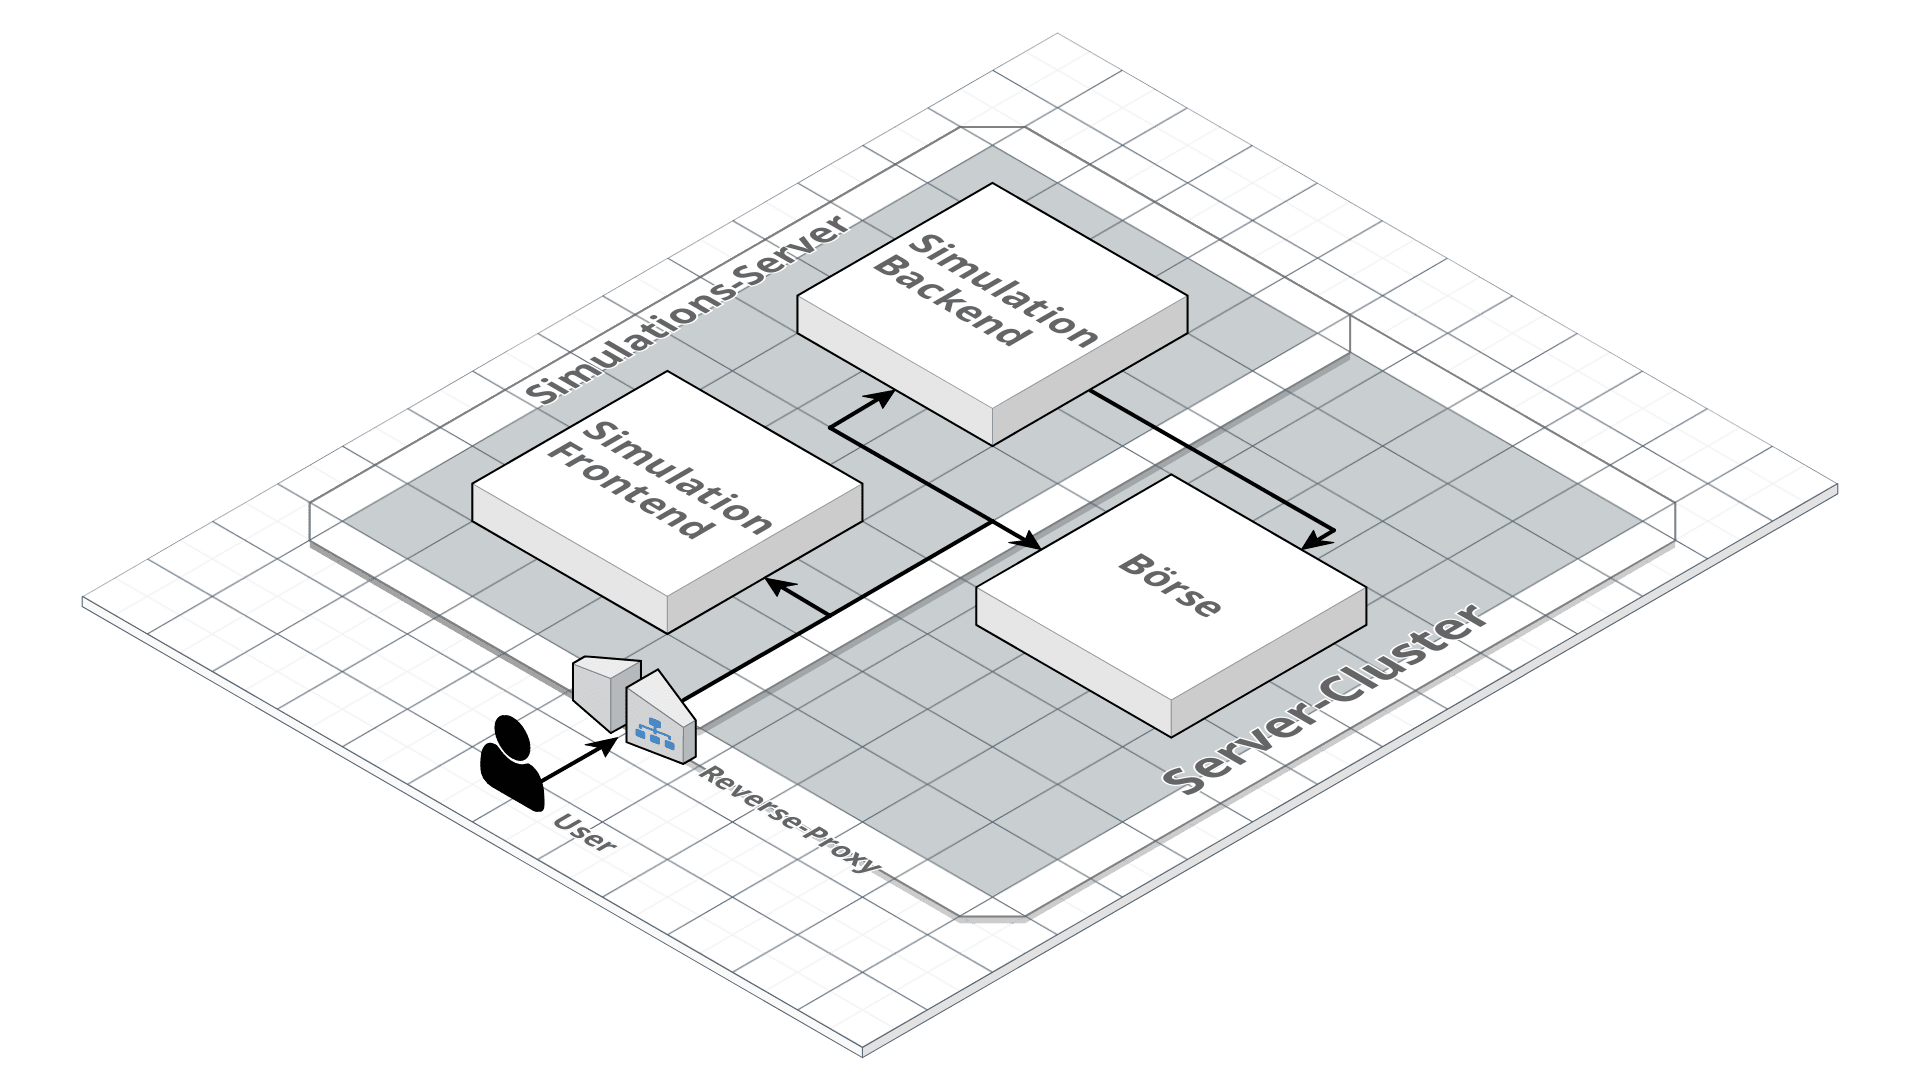
\includegraphics[width=\textwidth]{img/architecture.png}
    \centering
    \caption{Architektur}
    \label{fig:architecture}
\end{figure}

In \autoref{fig:architecture} ist die Architektur der Anwendung dargestellt.
Alle benötigten Server sind in einem Server-Cluster organisiert.
Hier werden die Börse, die Kernlogik der Simulation ausgeführt und das Nutzerinterface an den User ausgeliefert. Zentralles Eintrittstor ist dabei ein Reverse-Proxy, welcher die Aufgabe hat, die Daten an die richtigen internen Server weiterzuleiten und Daten, die für den Nutzer sind zu verschlüsseln.
Innerhalb des Clusters kommunizieren der Simulations-Backend-Server direkt mit der Börse. Dadurch kann dieser Verkehr nicht von außen beeinflusst werden und mögliche Aktieninformationen (beispielsweiße wer welche Aktie handelt) sind geschützt.

Das Simulations-Frontend dient als grafische Benutzeroberfläche, mit dem das eigentliche Simulations-Backend gesteuert wird. Weitere Informationen dazu finden sich in \autoref{cha:Nutzerhandbuch}.

Unsere Architektur trennt dabei streng die Szenario-Logik vom Nutzerinterface.
Hat der Nutzer ein Szenario ausgewählt, alle Einstellungen getroffen und das Szenario gestartet, wird eine Anfrage an den Simulations-Backend-Server gesendet. Darauf hin beginnt dieser das entsprechende Szenario auszuführen und mit der Börse zu handeln.
Dies hat ein paar Vorteile gegenüber der Implementierung sämtlicher Logik innerhalb des Nutzerinterfaces:
\begin{enumerate}
    \item Zentralle Nutzersteuerung\\
        Der Backend-Server kann Ausführungen von Szenarios steuern. So werden beispielsweiße Kollisionen vermieden, wenn mehrere Szenarios von verschiedenen Nutzern gestartet werden würden.
    \item Code-Qualität\\
        Durch die Trennung der Logik nach dem Separation-of-Concern und Clean-Code Methodiken wird der Quelltext wartbarer.
    \item Unterbrechungen\\
        Der Nutzer kann ein Szenario starten, welches eine längere Dauer hat (z.\,B. mehrere Tage). Anschließend muss er nicht seinen COmputer eingeschaltet lassen. Das Szenario wird im Hintergrund ausgeführt.
\end{enumerate}

\section{Szenario}

\section{User Interface}
//TODO:
